\section{Construcción}
\subsection{Diseño PCB}

\subsubsection{Modulo de carga de batería}
Dentro de nuestro sistema para la prevención de muerte de cuna, es critico el monitoreo del lactante, para ello se utilizó una pila de litio, pero para que sea constante se implementó un módulo de carga TP4056.

Nuestro sistema de prevención trabaja con 3.3v y las pilas de litio sus voltajes son de 3.6v para lo cual se tiene que implementar un LDO.

\textbf{TP4056}

El TP4056 es un chip encapsulado en formato SOP-8 que es capaz de gestionar la carga de una batería. Es decir, adecua la entrada de energía para el estándar de 1A de la mayoría de las baterías de litio que se usan en la industria electrónica.

\textbf{LDO}

Un regulador de baja caída o LDO es un regulador de voltaje lineal de DC que puede regular el voltaje de salida cuando el voltaje de alimentación está muy cerca del voltaje de salida.

Los módulos comerciales no cuentan con este LDO, por lo cual se diseñó el esquemático para implementarlo a nuestro sistema.

\begin{figure}[htp!]
    \centering
    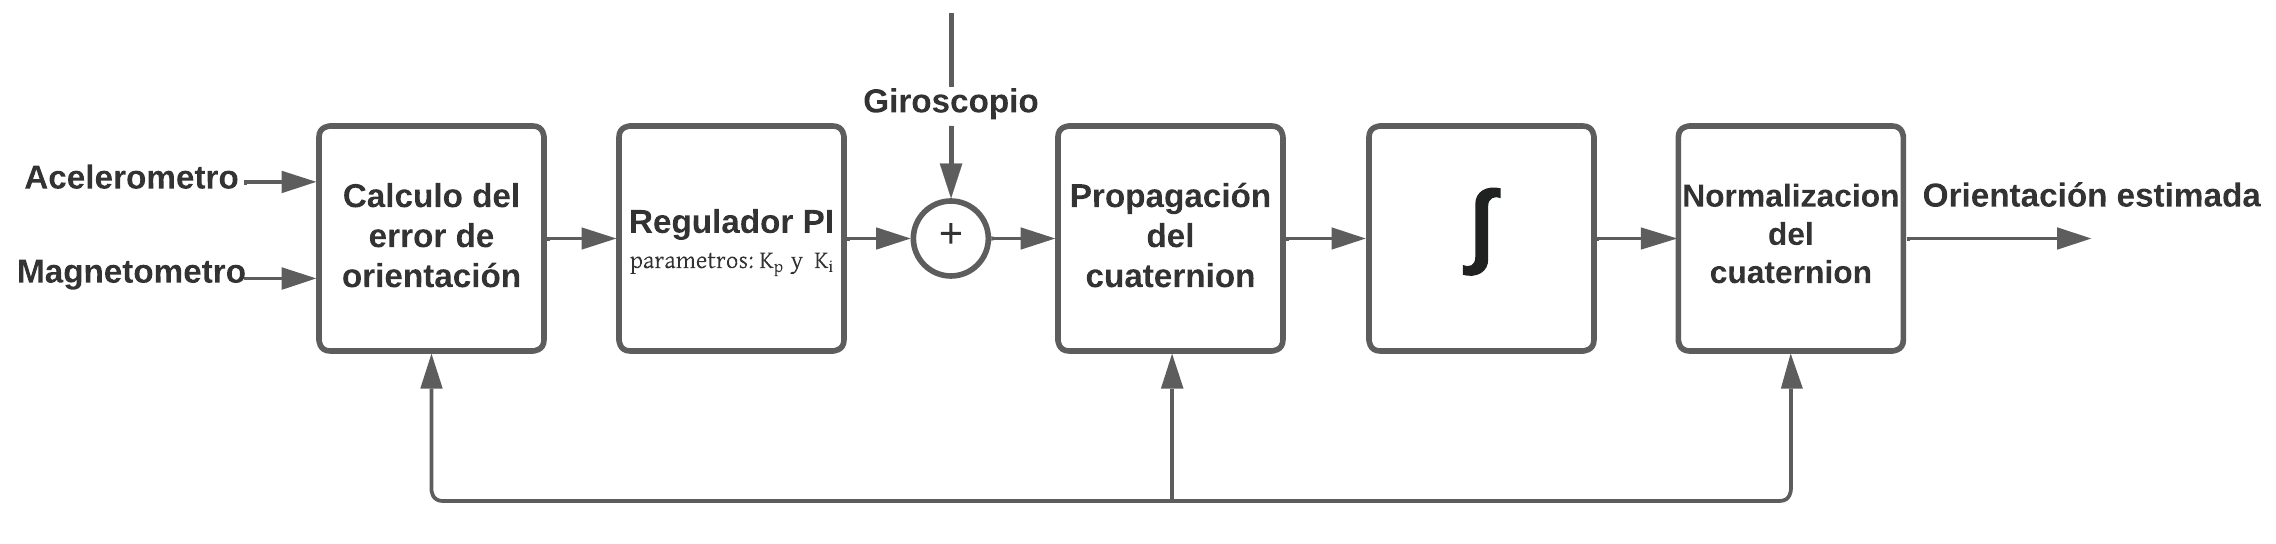
\includegraphics[width=\columnwidth]{bateria_squematic.jpg}
    \caption{Esquemáticos del módulo de carga de batería}
    \label{fig: bateria}
\end{figure}\FloatBarrier

\subsubsection{Layout}

Al diseñar los diagramas esquematicos y realizando las pruebas pertinentes se decidio realizar una unica pcb la cual seria de manera pequrña y que no represntara problemas o imcomodidad al lactante.

Se diseño un modelo 3D para poder corraborar de que tamaño quedaria nuestro dispositivo.

Todo esto diseñado en el software altium acontinuacion se muestran algunas imagenes del layout y el diseño 3D.
\begin{figure}[htp!]
    \centering
    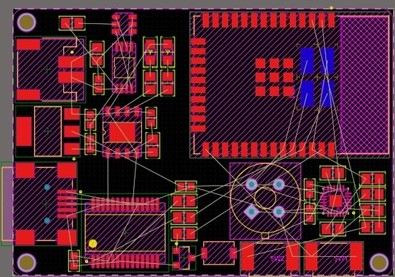
\includegraphics[width=\columnwidth]{layout.jpg}
    \caption{Layout de nuestro PCB}
    \label{fig: Layout}
\end{figure}\FloatBarrier

\subsubsection{PCB 3D}

\begin{figure}[htp!]
    \centering
    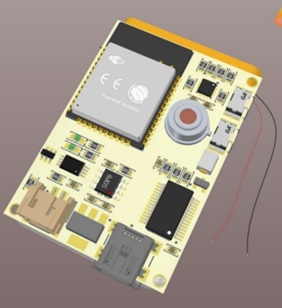
\includegraphics[width=\columnwidth]{vista_frontal_3D.jpg}
    \caption{Vista frontal PCB}
    \label{fig: frontal}
\end{figure}\FloatBarrier
\begin{figure}[htp!]
    \centering
    \includegraphics[width=\columnwidth]{vista_lateral_3D.jpg}
    \caption{Vista lateral PCB}
    \label{fig: lateral}
\end{figure}\FloatBarrier
\subsection{Carcasa}